\begin{figure}[!htb] 
\centering 
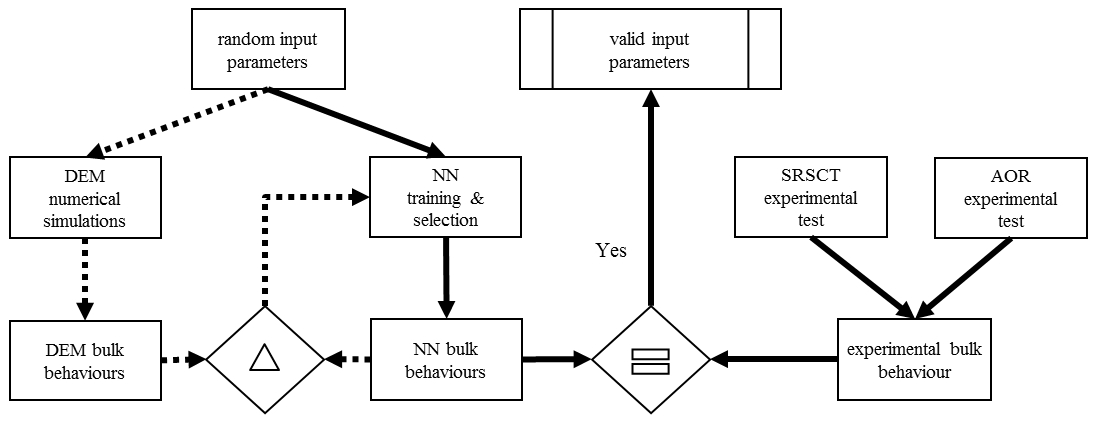
\includegraphics[width=.96\textwidth]{images/original/19methodology} 
\caption[Methodology]{Methodology. 
In the training phase (dashed line) from the initial random input parameters
$DEM$ simulations are performed. The behaviours provided are used to train the
Neural Networks ($NN$), in a loop that continues until the difference is within
the limit ($\Delta$).
Then we identify the valid input parameters by comparing (\textbf{=}) $NN$ and
experimental behaviours in the parameters' identification phase (straight line).
Further explanations in the text.
}
\label{fig:19methodology} 
\end{figure}


% \begin{figure}[htp]
%     \centering
%     
\includegraphics[width=.2\textwidth]{images/vitae/lbenvenuti}
%     \caption{OpenMP, MPI, MPI/OpenMP Hybrid runs of Box in a box testcase on 32
%     cores. The OpenMP-only run suffers from limited memory bandwidth in
%     memory-bound algorithms inside of the Modify section of the code. MPI-only has
%     low averaged runtimes for each section, but a very large Other timing, which
%     hints for a large amount of load-imbalance. Hybrid timings are a bit worse
%     on average, but because of better balancing, processes have lower wait times
%     inside of Other timing.}
% 	\label{fig:boxInBoxComparison}



% After the $DEM$ simulations the Neural
% Network ($NN$) are trained and selected. We then compare experimental and
% numerical results to identify the valid parameters.